\subsection{Любой частичный порядок можно дополнить до линейного}

\textbf{Применение леммы Цорна: любой частичный порядок можно дополнить до линейного.}\\

Если $P$ -- отношение частичного порядка, то существует $S$ -- отношение линейного порядка, т.ч. $P \subset S$. 
В качестве $A$ рассмотрим множество отношений порядка. Упорядочение на $A$ -- вложение как подмножества. 
Это упорядочение соответствует условию леммы Цорна: у любой цепи есть верхняя грань, а именно объединение всех элементов цепи.\\

Нужно доказать, что в объединении получится порядок: \\

\textbf{Рефлексивность :} наследуется из каждого элемента цепи 

\textbf{Антисимметричность :} если в итоговом порядке $a < b$ и $b < a$, то для каких-то порядков из цепи $a \leq_i b, b \leq_j a$:

Если $j > i$, то $a \leq_j b$. Из антисимметричности $\leq_j$ ‚ Получаем $a = b$. 

\textbf{Транзитивность :} аналогично, если $a \leq b$ и $b \leq c$, то $a \leq_i b$ и $b \leq_j c$, отсюда $a \leq_j b, b \leq_j c$, откуда $a \leq_j c$ и потому $a \leq c$\\

По лемме Цорна есть максимальный элемент. Нужно доказать, что он линеен. 
Т.е. если какие-то $2$ элемента не сравнимы, то порядок можно продолжить. 

Пусть $a$ и $b$ несравнимы. 
Тогда построим новый порядок $x \leq^{'} y$, если $\begin{bmatrix}
    x \leq y \\
    x \leq a, b \leq y
\end{bmatrix}$\\

Докажем, что $\leq^{'}$ является порядком. 

Рефлексивность : наследуется из $\leq$ 
Антисимметричность. 4 случая.\\

Если $x \leq y$ и $y \leq x$, то $x = y$ по антисимметричности $\leq$.

Если $x \leq y, y \leq a, b \leq x$, то $b \leq a$, что противоречит предположению.

Остальные два случая аналогичны.\\

Транзитивность:\\

Если $x \leq y, y \leq a, b \leq z$, то $x \leq a, b \leq z \Rightarrow x \leq^{'} z$

Если $x \leq a, b \leq y, y \leq a, b \leq z$, то $b \leq a$, что невозможно.\\

Получаем, что все 3 свойства верны. 
Т.е. нелинеиный порядок можно дополнить, поэтому максимальный элемент является линейным.

\subsection{Объединение двух бесконечных множеств равномощно одному из них.}

\textbf{Вспомогательная теорема. Формулировка:}  Если $A$ бесконечно, то множество $A \times N$ равномощно $A$. \\

\textbf{Доказательство:} Вполне упорядочим множество $A$. Мы уже знаем, что всякий элемент множества $A$  однозначно представляется в виде $z + n$, где $z$ --  предельный элемент (не имеющий непосредственно предыдущего), а $n$ -- натуральное число. Это означает, что $A$ равномощно $B \times N$, где $B$ -- множество предельных элементов. (Тут есть небольшая трудность --  последняя группа элементов конечна, если в множестве есть наибольший элемент. Но мы уже знаем, что добавление конечного или счётного множества не меняет мощности, так что этим можно пренебречь.) Теперь утверждение теоремы очевидно: $A \times N$ равномощно $(B \times N) \times N$, то есть $B \times (N \times N)$ и тем самым $B \times N$ (произведение счётных множеств счётно), то есть $A$. \\

По теореме Кантора-Бернштейна отсюда следует, что промежуточные мощности (в частности, $|A|+|A|$, а также любое произведение $A$ и конечного множества) совпадают с $|A|$. \\

\textbf{Формулировка: } Сумма двух бесконечных мощностей равна их максимуму. 
\textbf{Доказательство: } Прежде всего напомним, что любые две мощности сравнимы. Пусть, скажем,$|A| \leq |B|$. Тогда$|B| \leq |A|+|B| \leq |B|+|B| \leq |B| \times \mathbb{N} \leq |B|$ (последнее неравенство — утверждение предыдущей теоремы). Остаётся воспользоваться теоремой Кантора–Бернштейна и заключить, что $|B|=|A + B|$.

$B \preceq A, A \preceq A \cup B \preceq A \times {0, 1} \preceq A \times N \preceq A$

\subsection{Декартов квадрат бесконечного множества равномощен ему.}

\textbf{Доказательство: } Заметим, что для счётного множества мы это уже знаем. Поэтому в $A$ есть подмножество, равномощное своему квадрату. Рассмотрим семейство всех таких подмножеств вместе с соответствующими биекциями. Элементами этого семейства будут пары $(B, f)$, где $B$ -- подмножество $A$, а $f: B \to B \times B$ -- взаимно однозначное соответствие. Введём на этом семействе частичный порядок: $(B_1, f_1) \leq (B_2, f_2)$, если $B_1 \subset B_2$ и ограничение отображения $f_2$ на $B_1$ совпадает с $f_1$.

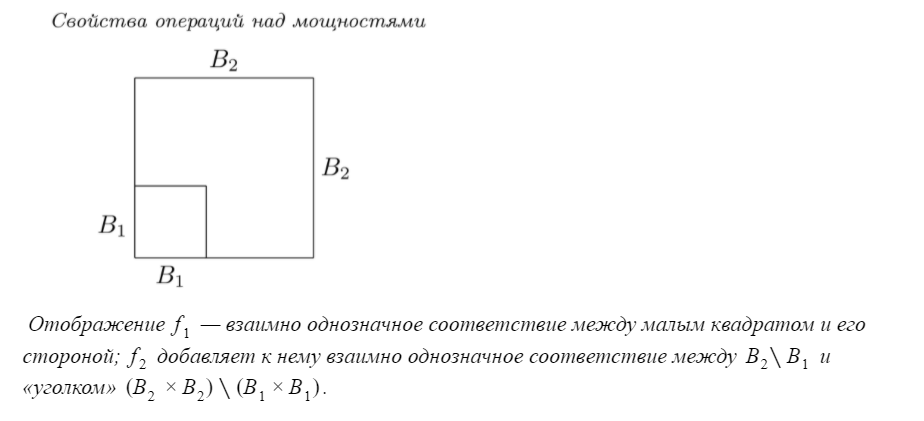
\includegraphics{images/2.12 1.png}

Теперь применим лемму Цорна. Для этого нужно убедиться, что любое линейно упорядоченное (в смысле описанного порядка) множество пар указанного вида имеет верхнюю границу. В самом деле, объединим все первые компоненты этих пар; пусть $B$ — их объединение. Как обычно, согласованность отображений (гарантируемая определением порядка) позволяет соединить отображения в одно. Это отображение (назовём его $f$) отображает $B$ в $B \times B$. Оно будет инъекцией: значения $f(b')$ и $f(b'')$ при различных $b'$ и $b''$ различны (возьмем большее из множеств, которым принадлежат $b'$ и $b''$; на нём $f$ является инъекцией по предположению). С другой стороны, $f$ является сюръекцией: для любой пары $(b', b'') \in B \times B$ возьмём множества, из которых произошли $b'$ и $b''$, выберем из них большее и вспомним, что мы имели взаимно однозначное соответствие между ним и его квадратом.\\

По лемме Цорна в нашем частично упорядоченном множестве существует максимальный элемент. Пусть этот элемент есть $(B, f)$. Мы знаем, что $f$ есть взаимно однозначное соответствие между $B$ и $B \times B$ и потому $|B| = |B| \times |B|$. Теперь есть две возможности. Если $B$ равномощно $A$, то $B \times B$ равномощно $A \times A$ и всё доказано. Осталось рассмотреть случай, когда $B$ не равномощно $A$, то есть имеет меньшую мощность (большей оно иметь не может, будучи подмножеством). Пусть $C$ -- оставшаяся часть $A$, то есть $A \backslash B$.

Тогда $|A| = |B| + |C| = max(|B|, |C|)$, следовательно, $C$ равномощно $A$ и больше $B$ по мощности. Возьмём в $C$ часть $C'$, равномощную $B$, и положим $B' = B + C'$.

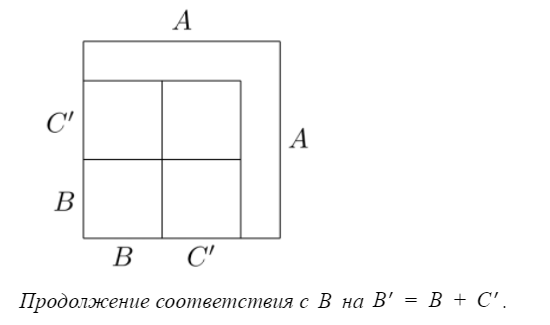
\includegraphics{images/2.12 2.png}

Обе части множества $B'$ равномощны $B$. Поэтому $B' \times B'$ разбивается на $4$ части, каждая из которых равномощна $B \times B$, и, следовательно, равномощна B (т.к. $C', (B' \times B'), (B \times B)$  равномощны $B$). В итоге мы получаем большую пару $(B', f')$, что противоречит утверждению леммы Цорна о максимальности. Таким образом, этот случай невозможен.